\chapter{多态}

\section{多态}

\subsection{多态(Polymorphism)}

多态是同一个行为具有多个不同表现形式或形态的能力。

\begin{figure}[H]
	\centering
	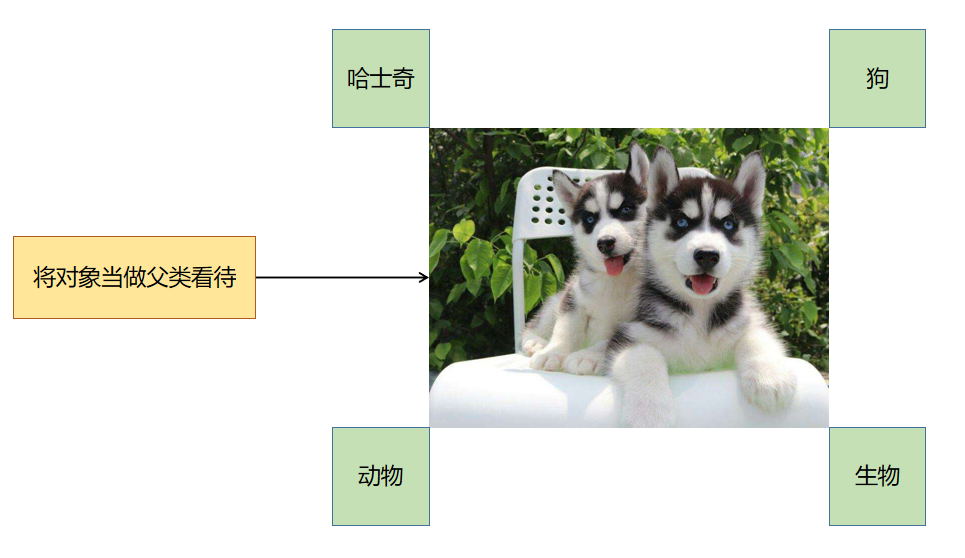
\includegraphics[scale=0.7]{img/C4/4-1/1.png}
	\caption{多态}
\end{figure}

\begin{figure}[H]
	\centering
	\begin{tikzpicture}[]
		\draw (0,0) node {Animal animal = new Dog();};

		\draw (-3,-2) rectangle (-1,-1);
		\draw (1,-2) rectangle (3,-1);
		\draw (-2,-1.5) node {父类引用};
		\draw (2,-1.5) node {子类对象};

		\draw[->] (-2,-1) -- (-1.5,-0.3);
		\draw[->] (2,-1) -- (1.5,-0.3);
	\end{tikzpicture}
	\caption{父类引用指向子类对象}
\end{figure}

通过父类引用指向子类对象,从而产生多种形态。父类引用仅能访问父类所声明的属性和方法,不能访问子类独有的属性和方法。 \\

在一对有继承关系的类中都有一个方法,其方法名、参数列表、返回值均相同,通过调用方法实现不同类对象完成不同的事件。 \\

构成多态需要满足三个条件:

\begin{enumerate}
	\item 必须存在继承关系。
	\item 继承关系中必须有同名的虚函数。
	\item 存在基类类型的指针或引用,通过该指针或引用调用虚函数。
\end{enumerate}

\newpage

\section{虚函数}

\subsection{虚函数}

